\section{Examples of applications for Monte Carlo simulations}
\label{sec:examples}
%guardare:

%~\cite{Sarrut2018} Sarrut D, Krah N, Badel JN, Létang JM. Learning SPECT detector angular response function with neural network for accelerating Monte-Carlo simulations. Phys Med Biol 2018;63. https://doi.org/10.1088/1361-6560/aae331.

%~\cite{Sarrut2019}
%Sarrut D, Krah N, Létang JM. Generative adversarial networks (GAN) for compact beam source modelling in Monte Carlo simulations. Phys Med Biol 2019;64:215004. https://doi.org/10.1088/1361-6560/ab3fc1.

%~\cite{Sadeghnejad-Barkousaraie2020}
%Sadeghnejad-Barkousaraie A, Bohara G, Jiang S, Nguyen D. A reinforcement learning application of guided Monte Carlo Tree Search algorithm for beam orientation selection in radiation therapy. ArXiv 2020. https://doi.org/10.1088/2632-2153/abe528.

%~\cite{Liu2020a} 
%Liu CC, Huang HM. A deep learning approach for converting prompt gamma images to proton dose distributions: A Monte Carlo simulation study. Phys Medica 2020;69:110–9. https://doi.org/10.1016/j.ejmp.2019.12.006.

%~\cite{Peng2019}
%Peng Z, Shan H, Liu T, Pei X, Zhou J, Wang G, et al. Deep learning for accelerating Monte Carlo radiation transport simulation in intensity-modulated radiation therapy. ArXiv 2019:1–8.

%\cite{Ma2020c}
%Ma S, Hu Z, Ye K, Zhang X, Wang Y, Peng H. Feasibility study of patient-specific dose verification in proton therapy utilizing positron emission tomography (PET) and generative adversarial network (GAN). Med Phys 2020;47:5194–208. https://doi.org/10.1002/mp.14443.



%\subsection{Emulation of electromagnetic interaction models}

\subsection{Emulation of radiation-matter interactions}
\label{subsec:interactions}
%tommaso
% computational cost of full fledged simulations; their not complete ability to match data
One of the most complex tasks in Monte Carlo simulations involving the use of detectors (medical apparatuses, particle physics detectors) lies in the dual need of being able to optimize the design before detector construction, and to simulate the behavior under working conditions after the setup has been prepared.
In both cases, unless the setup is very similar to existing detectors, extensive Monte Carlo simulations of the expected detector capabilities are the widely used solutions. Various such tools exist (Geant4~\cite{Agostinelli2003}, Fluka~\cite{Bohlen2014}, MCNPX~\cite{Hughes2001}), with different application regimes and specific utilization patterns. As a general rule, these implement iteratively basic radiation-matter low-level processes to a knowledge of the detector setup, including materials, geometry and  other experimental conditions; as such, they incur into two general limits:
\begin{itemize}
\item a scarce capability to be tuned to experimental results, by changing the basic modelling of the processes;
\item a large to very large need for computational resources, given the iteration oriented approach and the need to increase the level of iterations in order to obtain a better precision and adherence to data.
\end{itemize}

% Geant4, Fluka, MCNPX: https://doi.org/10.1063/1.2720459

Both limitations can in principle be surpassed via the use of Artificial Intelligence oriented tools.
In presence of experimental data, the response of the AI system can be tuned to that without any explicit modelling of the physics processes; speed can be vastly improved by the change from iteration-based computations to standard Deep Learning matrix algebra, with its intrinsic capabilities for high performance processing on, for example, GPU systems.

As an example, we want to consider here CaloGan~\cite{Paganini2018}, an attempt to reproduce the details of radiation-matter interactions in the complex setup of segmented (3 layers) electromagnetic calorimeters.
A Generative Adversarial Network, as those presented in Section~\ref{subsec:gan}, is used in conjunction with an as-accurate-as-possible Geant4 simulation of the same experimental setup. The generator side accepts in input particles' 4-momenta, and, after the passage through quite standard convolutional (matching the detector response as 2-D images) and dense layers, the output is compared with detailed Geant4 simulations of particles with the same parameters.  The training optimizes the energy deposition per layer and per 2-D transverse cell, in a way in principle suited also for using real data in input. Results are very encouraging, even in an extreme detector scenario: not only the quantities of direct training are well reproduced, but also secondary and derived quantities like shower shapes are in most cases well described.

Results are shown in Figure~\ref{fig:calogan} for the explicit targets of the calculation (2-D layered images of the energy deposits, in the specific case of incoming positrons).


\begin{figure}[h]
    \centering
    \begin{subfigure}[b]{0.55\textwidth}
    \centering
    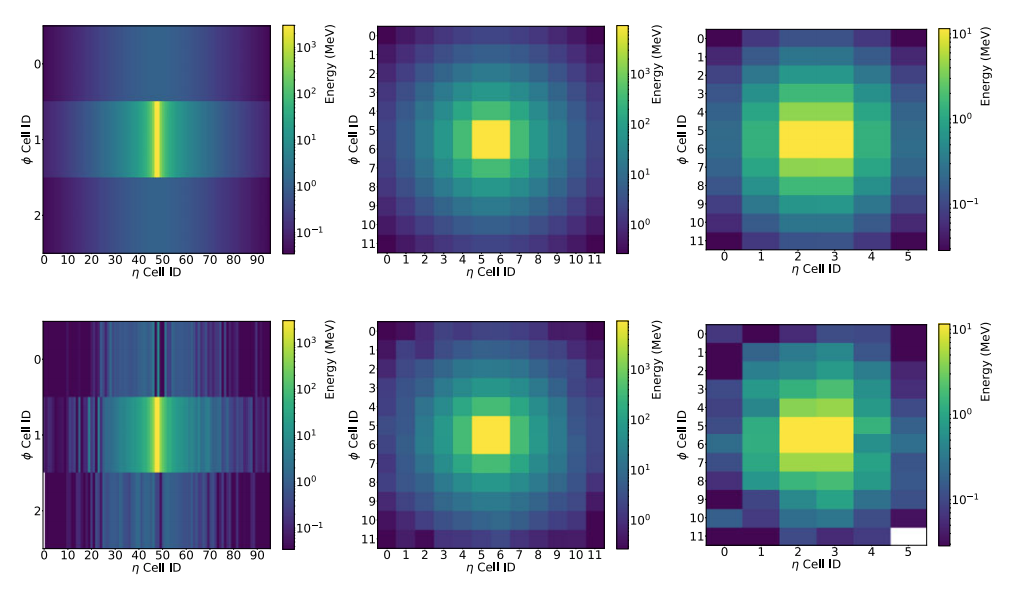
\includegraphics[width=1\textwidth]{images/calogan1.png}
    \end{subfigure}
    \hfill
        \begin{subfigure}[b]{0.44\textwidth}
        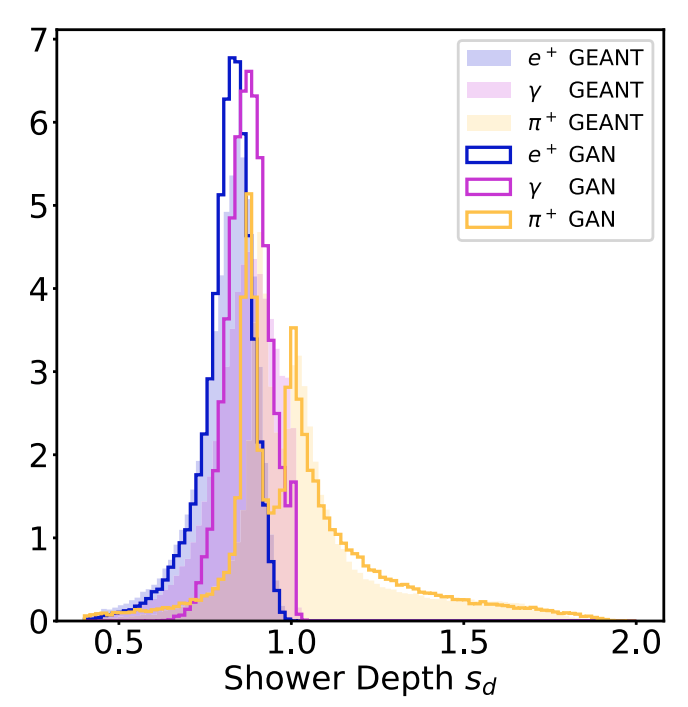
\includegraphics[width=1\textwidth]{images/calogan2.png}
        \end{subfigure}
\caption{(left) Average e$^+$ Geant4 shower (top), and average e$^+$
CALOGAN shower (bottom), with progressive calorimeter depth
(left to right). (right) Energy weighted shower depth (in a.u.) from CaloGan and Geant4 detailed simulations. (From~\cite{Paganini2018}).}
        \label{fig:calogan}
\end{figure}


Interestingly, one can look into quantities derived from shower shapes, but not directly targeted by the GAN training step, like for example the energy weighted shower depth. As we will see in Section~\ref{subsec:speed}, in general one cannot assume these quantities will be perfectly reproduced; in this specific case, though, the agreement level is quite impressive.


A second similar attempt, applied to the not-yet existing CLIC proposed electromagnetic and hadronic calorimeter, is presented in~\cite{Carminati2018}, with the goal to directly reproduce 3-D signals in a highly granular calorimeter. The reference dataset, in absence of real data, has the form of Geant4 generated showers sampled in a 25x25x25 cells around the impinging particle.
% https://doi.org/10.1051/epjconf/201921402010
Figure~\ref{fig:3dgan}(left) shows the longitudinal shower shapes for 100 GeV electrons in the electromagnetic part of the calorimeter compared with detailed Geant4 simulations. The level of agreement is very satisfactory. Figure~\ref{fig:3dgan}(right) shows a pictorial rendering of the expected energy deposit by a 100 GeV electron in the calorimeter.



\begin{figure}[h]
    \centering
    \begin{subfigure}[b]{0.54\textwidth}
    \centering
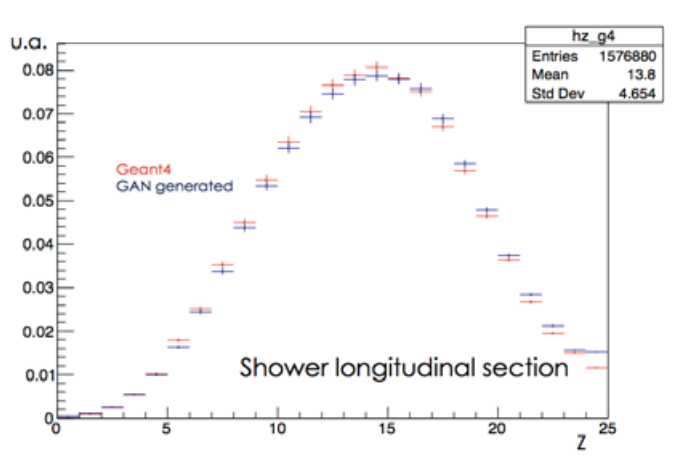
\includegraphics [width=\textwidth]{images/3dgan.png}
    \end{subfigure}
    \hfill
        \begin{subfigure}[b]{0.44\textwidth}
        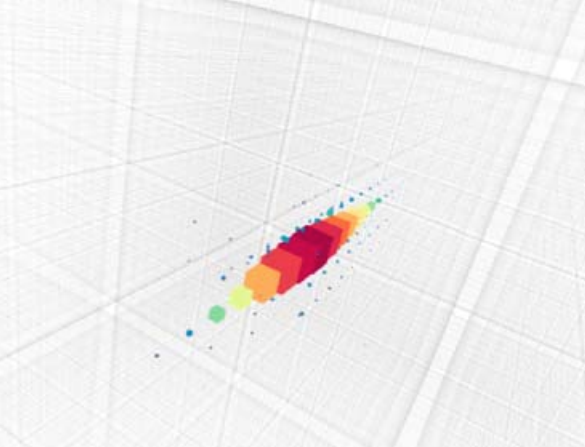
\includegraphics [width=\textwidth]{images/3dgan1.png}

        \end{subfigure}
        \caption{(left) Longitudinal shower shapes for 100 GeV electrons: GAN result is compared to full Geant4
simulation. The Z coordinate indicates the bin index in the longitudinal direction. (right) The three-dimensional representation of an energy shower created by a 100
GeV electron as generated by the GAN, using particle type as conditioning information. (From \cite{Carminati2018}).}
        \label{fig:3dgan}

\end{figure}

In sections~\ref{subsec:speed} and ~\ref{subsec:physical} we will discuss about the speed gain with respect to standard methods, and solutions and needs to prevent unphysical results.

%CM aggiungerei una frase sulle potenziali applicazioni mediche
The last two examples are related to High-Energy particle Physics, however, a similar approach can be used also to emulate the energy deposition in a voxel geometry, such as the CT of a patient.

In the field of hadron therapy, strong requirements are imposed on the accuracy in predicting the range of the treatment field in patients, and the development of patient specific dose verification methods is highly desired. Positron Emission Tomography (PET) imaging can be used to monitor the activity generated in the body tissues by the interaction with the therapeutic hadronic beams. Attempt to establish the correlation between the activity measured with a PET detector and the dose released to tissues have been carried out by utilizing  machine learning techniques based on RNN in the study by Hu et al.~\cite{Hu2020} and on GAN in the study by Ma et al.~\cite{Ma2020c}. Imaging the prompt gamma radiation is another approach to dose monitoring in hadron therapy. A deep learning based conversion of the prompt gamma information into proton dose distribution has been proposed by Liu et al~\cire{Liu2020a}. 


\subsubsection{Emulation of detector responses}
Monte Carlo tools like Geant4 are designed to simulate, as accurately as possible, the energy deposition (in keV, for example) due to the passage of particle / radiation in the material of a detector. In real life, what a scientist measures is instead the response, as analog or digital signals, of a measuring device in which energy deposition is read and processed by some electronic boards. In classical systems, the simulation of radiation / matter must be followed by an ad-hoc simulation of the electronic readout system, in order to be compared with actual readings from a detector. In the case of AI inspired tools, this can be avoided by completely bypassing the ``energy deposition'' output results, and training the system directly with real or realistic (from the above ad-hoc simulation) signals from the electronic back-end  (see Figure~\ref{fig:elec}).
%In~\cite{mri}, for example, images from a real MRI apparatus are used for the training the system (see Figure~\ref{fig:elec}); 
%the use of more classical approaches would be indeed more problematic since there is no practical way to measure (and validate) the output in terms of energy deposition in a running system.

MC simulations are also frequently used to estimate the efficiency and the geometrical acceptance of a detector, or a  system of detectors. The simulation of a Single Photon Emission Computed Tomography (SPECT) is usually done in two steps: the first one simulates the interactions of the produced photons with the patient, producing as output the emerging photons; and the second one simulates the response of the collimator-detector system to the emerging photons. This second step is called Angular Response Function (ARF).
Sarrut et al.~\cite{Sarrut2018} used a GAN to emulate the ARF. The DL algorithm takes as input the incidence angles of the photon and its energy and gives back the probability of detecting it in one of the possible energy windows. %CM: in realta' ho letto che l'output di una rete simile non può essere considerata una probabilita'
In summary, the DL algorithm emulates the detector system, including the collimators.

\begin{figure}[h]
    \centering

    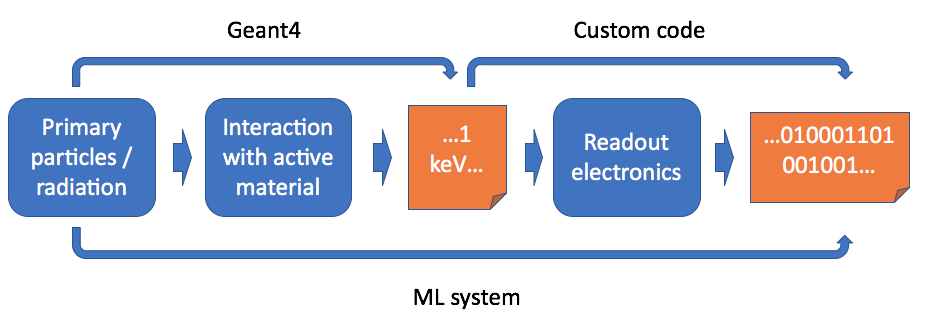
\includegraphics[width=0.8\textwidth]{images/electronics.png}
    \caption{Difference between classical and AI inspired simulation of experimental setups.}
     \label{fig:elec}

\end{figure}

%ale: trovi tu una referenza decente questo
%tommaso

\subsection{Emulation of nuclear interaction models}
Nuclear reactions models are one of the most demanding part of a MC simulation in terms of running time. Despite the large running time, the models already available in toolkits made to develop MC simulation, such as Geant4, have shown severe limitations in reproducing experimental data below 100~MeV/u~\cite{Arce2021}. Models developed by theoreticians for this energy domain can be interfaced with Geant4 with good results~\cite{Mancini-Terracciano2019}, however their running time is even larger. Ciardiello et al.~\cite{Ciardiello2020} obtained encouraging preliminary results 
in emulating one of the state-of-the-art models for low energy nuclear reactions with a VAE. The model in question is BLOB (``Boltzmann-Langevin One Body'')~\cite{Napolitani2013}, which simulates the first part of the nuclear reaction, from the contact of the two nuclei until the energy of the nucleons composing the fragments is balanced among them. The BLOB output is a PDF of finding a nucleon in a given position of the phase space. The authors trained a VAE in reproducing the BLOB prediction in the interaction of two $^{12}$C nuclei at 62~MeV/u. For this purpose, they discretized and reduced the dimensionality of the BLOB output to use 3D convolutional layers. In detail, the dimensionality reduction uses the fact that in the reaction in exam BLOB predicts at most three large fragments, i.e. larger than one nucleon. Therefore, they divided the PDF produced by BLOB in three PDFs, one per large fragment, and associated all the nucleon emitted in the first part of the reaction to one of these three large fragments. In this way they used the three colour channels of convolutional layers to represent each of the possible large fragments. In spite of controlling the generative part, they trained a classifier for the event impact parameter ($b$) jointly with the VAE itself. This joint training helps the VAE in learning a the task, given the large sparsity of the input, and force the latent space in being organise with respect to the impact parameter. Moreover, it will be possible to sample from the latent space deciding the impact parameter of each generation.
Figure \ref{fig:out} shows that the VAE is able to generate PDFs very similar to the input one when sampling a point nearby the position in the latent space where the input has been encoded.

%\begin{figure}[!bht]
%\centering
%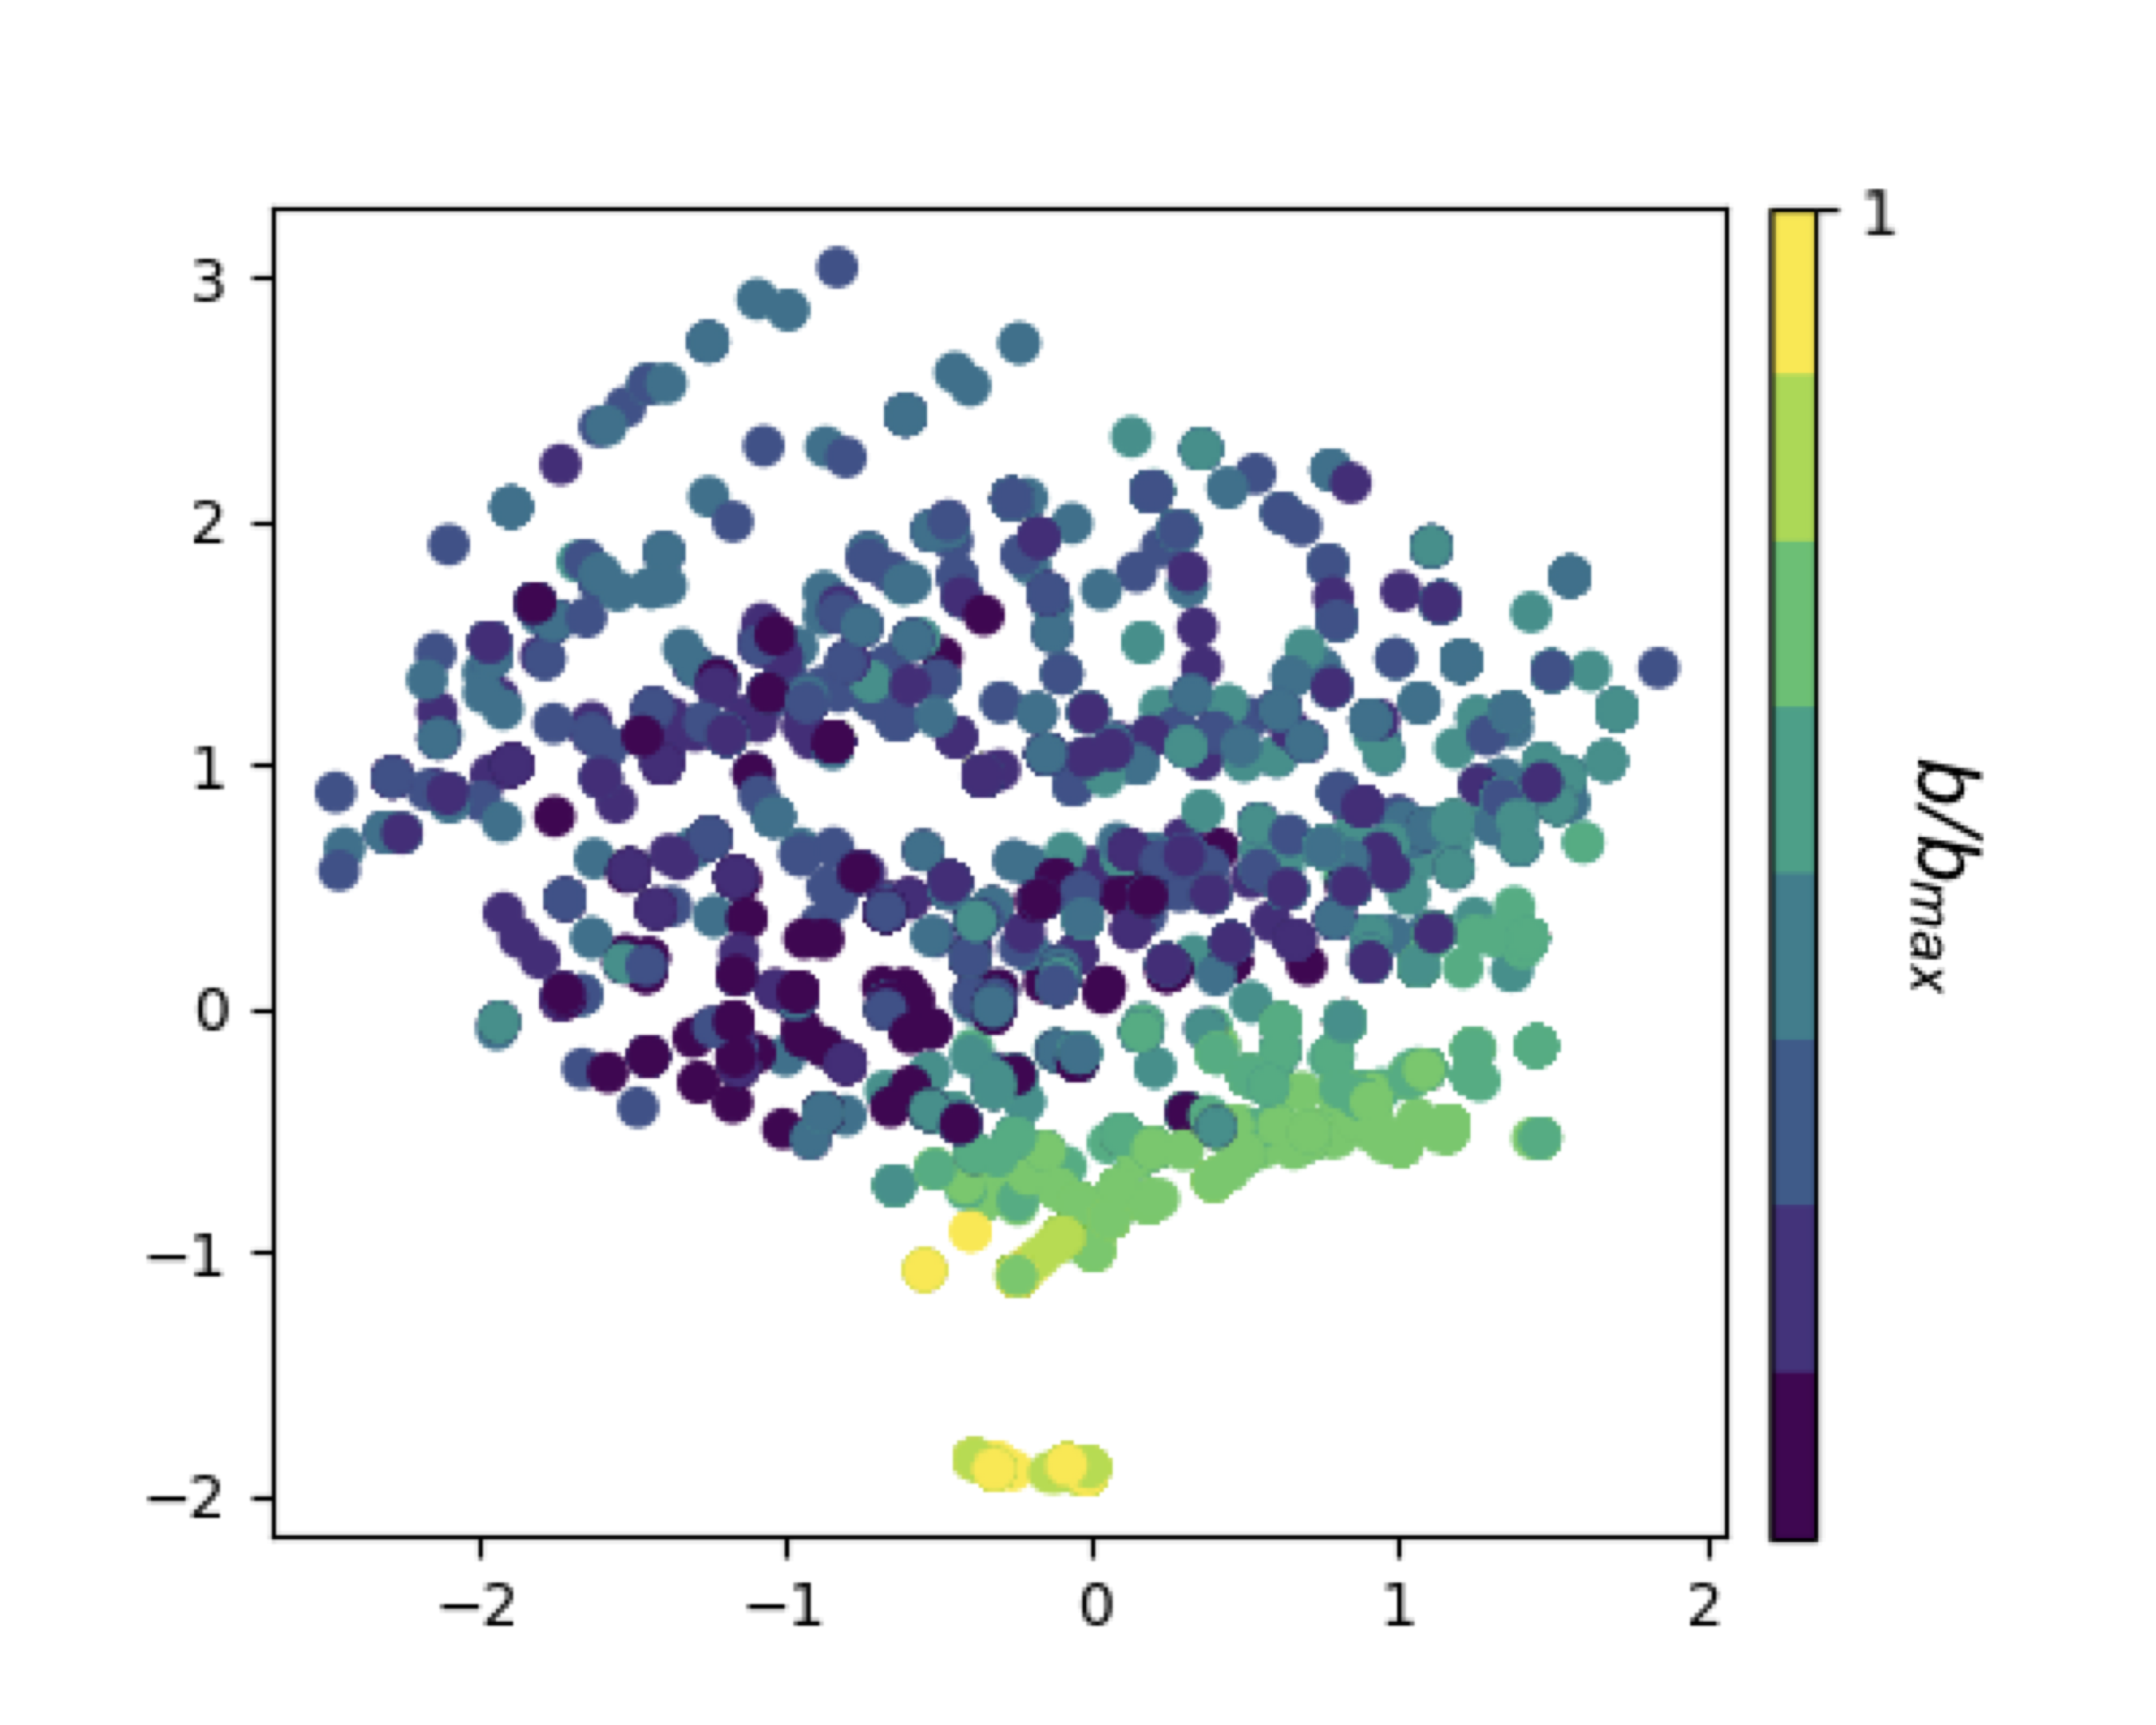
\includegraphics [width=.7\textwidth]{images/latent3}    
%\caption{Representation of the VAE latent space described in the text. Each point is the encoding point of one training %distribution, the color scale represent the impact parameter of the event.}
%\label{fig:latent}
%\end{figure}

\begin{figure}[!bht]
\centering
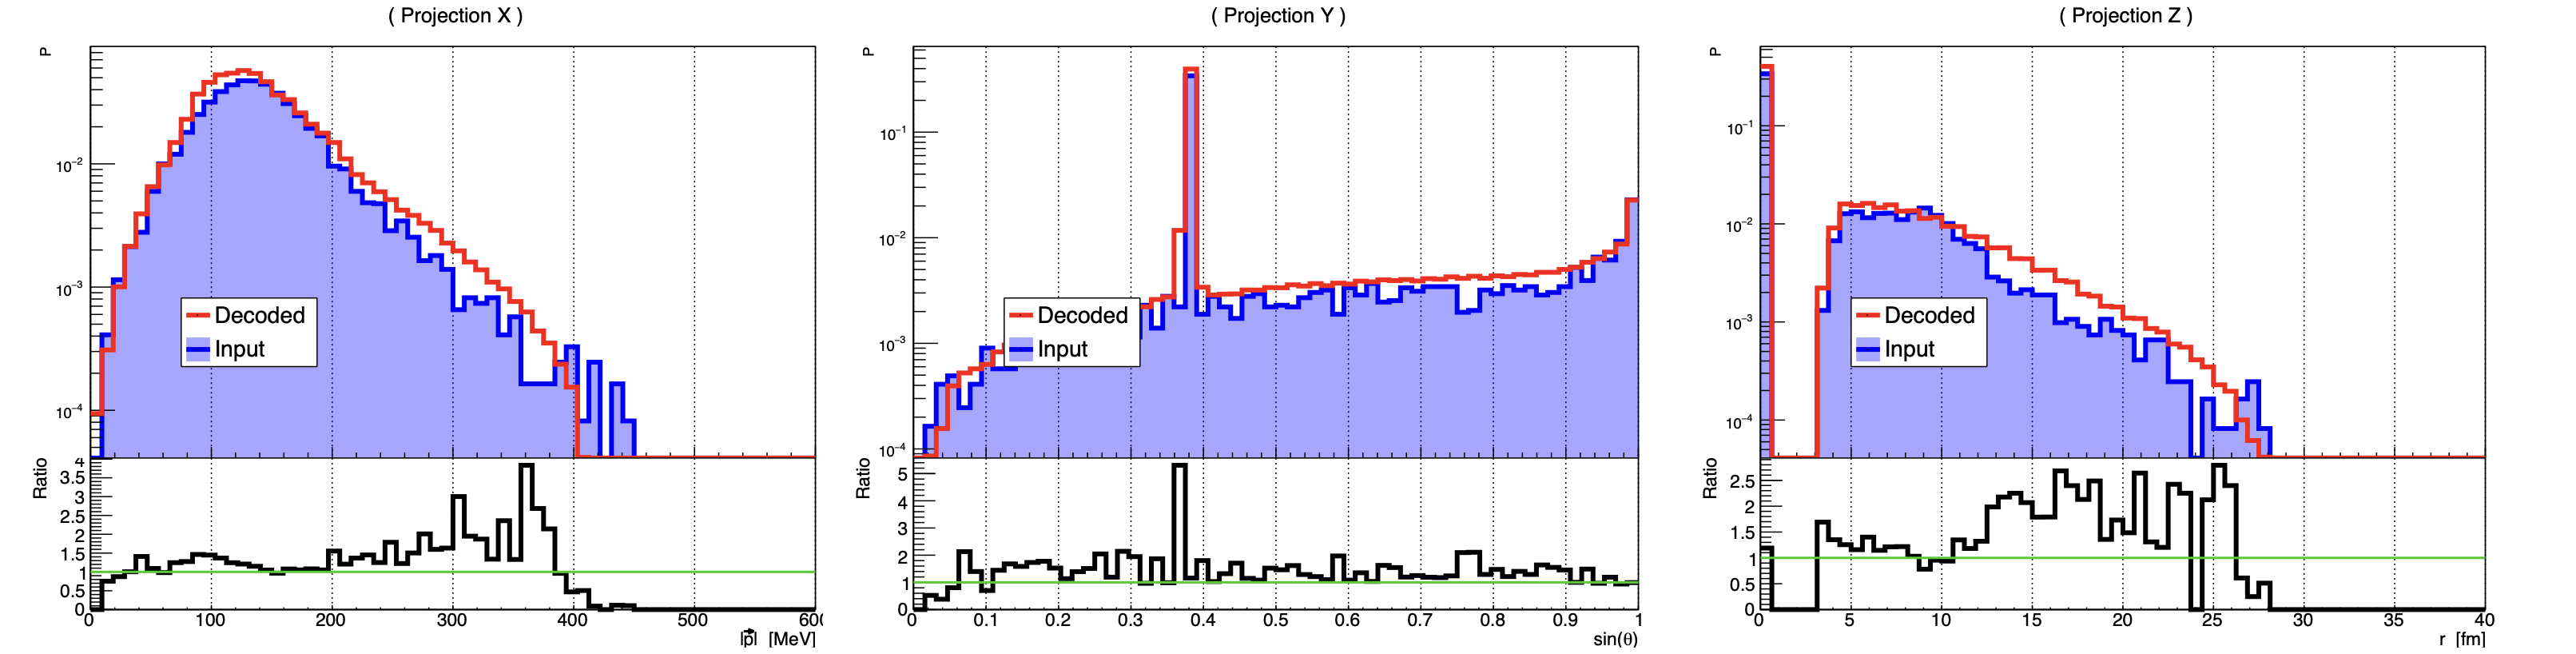
\includegraphics [width=\textwidth]{images/generated}
%\includegraphics [width=.9\columnwidth]{images/cy1}
%\includegraphics [width=.9\columnwidth]{images/cz1}
\caption{Example of results obtained in generating with the VAE a distribution, in red, starting from a point sampled from the neighborhood of the point where the input distribution, in blue, is encoded. The three distributions are the projections on the three axis of 3D PDFs.}
\label{fig:out}
\end{figure}

%They conclude their work planning to enlarge the VAE latent space and train the VAE with different projectile energies and using different ions as projectile and target besides interfacing the VAE decoder with Geant4,
% so that it will be possible to use BLOB
% for simulating low energy nuclear interactions without its computational overhead

%\begin{figure}[!bht]
%\centering
%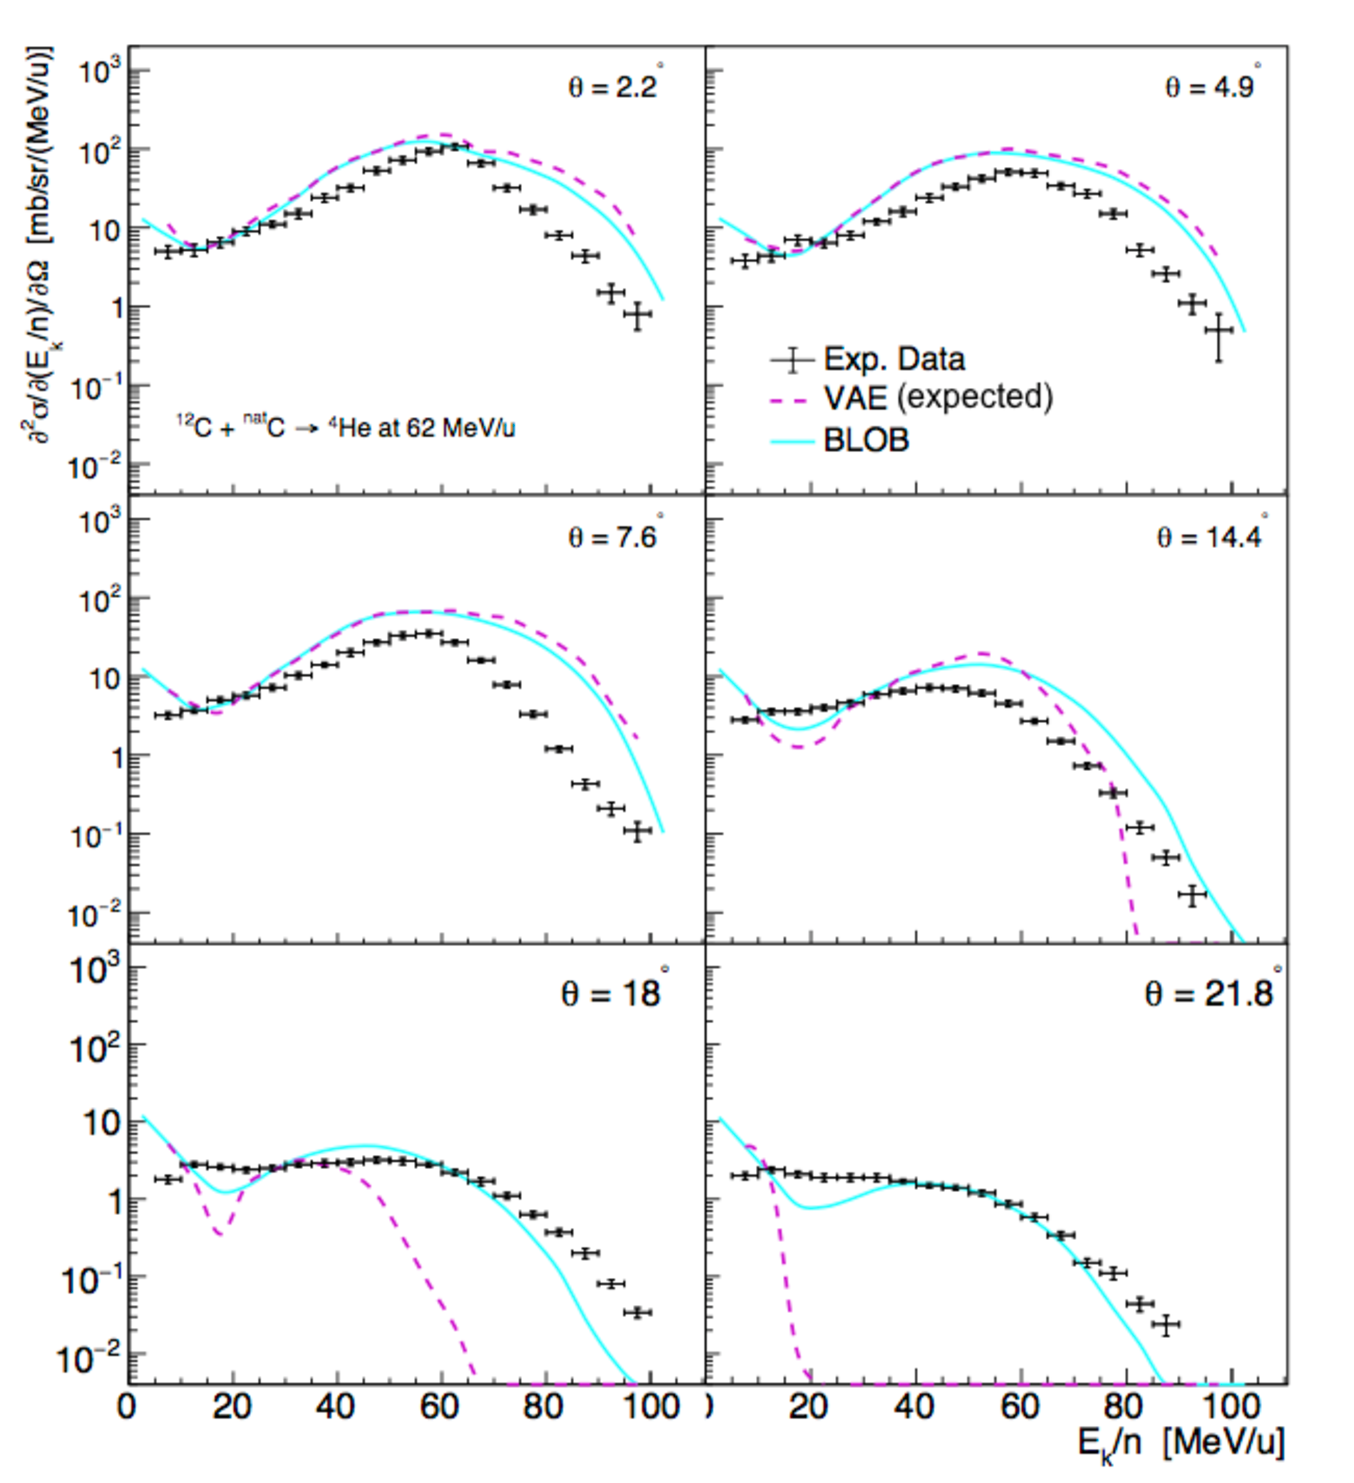
\includegraphics [width=.9\columnwidth]{images/test_reco}
%\caption{Double differential cross sections of alpha particle production in the reaction of $^{12}$C on a thin $^{12}$C target at 62~MeV/u as a function of the kinetic energy of the produced fragment for different angles. The experimental data, in black crosses, are from De Napoli et al.~\cite{DeNapoli:2012bs}. The continuous light blue lines show the BLOB predictions and the dashed magenta lines show the calculated values once encoded to reduce the PDF dimensionality and then decoded back.}
%\label{fig:testreco}
%\end{figure}

\subsection{A possible application of Graph Neural Networks}
To date, no specific study on Monte Carlo simulations of radiation / matter interactions using Graph Networks can be found in literature; still, it is clear from studies in other scientific domains suggest the potential of the technique. 
We want to cite here a study simulating the mechanical behavior of a fluid system, which shows capabilities of rendering the physics behind a complex system such as an ensemble of water small volumes~\cite{Sanchez-Gonzalez2020}; we expect similar GNN systems to become available for our research fields in short time.
